% Compile with LuaLaTeX (recommended) + BibTeX
%   latexmk -C
%   latexmk -lualatex -bibtex -interaction=nonstopmode -file-line-error acl_lualatex.tex
%
% Notes:
% - This file is self-contained: it auto-creates references.bib via filecontents.
% - Put all figures into ./figs/ with the exact filenames used below (or adjust names).
% - Underfull/Overfull \hbox warnings are usually harmless in ACL 2-column; errors are not.

% --- Ensure hyperref options are set BEFORE acl loads hyperref internally ---
\PassOptionsToPackage{
  colorlinks=true,
  linkcolor=blue,
  urlcolor=blue,
  citecolor=blue
}{hyperref}

\documentclass[11pt]{article}

% =========================
% ACL style (2-column)
% =========================
\usepackage[final]{acl}

\usepackage{titlesec}
\titlespacing*{\section}{0pt}{0.5\baselineskip}{0.3\baselineskip}
\usepackage{etoolbox}
\makeatletter
\makeatother

\makeatletter
\renewcommand{\bibsection}{\section*{References}}
\makeatother

% Đổi tên trong caption: Figure -> Hình, Table -> Bảng
\AtBeginDocument{%
  % cho caption (Figure/Table)
  \addto\captionsenglish{%
    \renewcommand{\figurename}{Figure}%
    \renewcommand{\tablename}{Table}%
  }%
  % cho autoref (Hình/Bảng/Mục)
  \renewcommand{\figureautorefname}{Figure}%
  \renewcommand{\tableautorefname}{Table}%
  \renewcommand{\sectionautorefname}{Section}%
  \renewcommand{\subsectionautorefname}{Section}%
}


% =========================
% Language & Fonts (VN/EN)
% =========================
\usepackage{fontspec} % explicit for XeLaTeX/LuaLaTeX stability
\usepackage[english,bidi=default]{babel}
\babelprovide[import]{vietnamese}

% Times-like fonts similar to ACL papers; safe mono font
\babelfont{rm}{TeX Gyre Termes}
\babelfont{sf}{TeX Gyre Heros}
\babelfont{tt}{Latin Modern Mono}
\babelfont[*vietnamese]{rm}{TeX Gyre Termes}

% =========================
% Quality / Lists
% =========================
\usepackage{microtype}
\usepackage{enumitem}
\setlist{itemsep=2pt,topsep=3pt}

% =========================
% Math / Tables / Figures
% =========================
\usepackage{amsmath,amsfonts,bm}
\usepackage{graphicx}
\usepackage{booktabs,multirow,tabularx}
\usepackage[table]{xcolor}
\usepackage{caption}
\captionsetup{font=small,labelfont=bf}
\captionsetup[figure]{name=Hình}
\captionsetup[table]{name=Bảng}
\usepackage{float}
\usepackage{placeins}
\usepackage{subcaption}

% Tell LaTeX where to look for assets
\graphicspath{{figs/}{assets/images/}{../plots/}{../assets/images/}}

% =========================
% TikZ (for diagrams)
% =========================
\usepackage{tikz}
\usetikzlibrary{shapes.geometric, shapes.symbols, arrows.meta, positioning, shadows, calc, fit, backgrounds}

\definecolor{userblue}{RGB}{52, 152, 219}
\definecolor{articlegreen}{RGB}{46, 204, 113}
\definecolor{socialorange}{RGB}{230, 126, 34}
\definecolor{cathub}{RGB}{155, 89, 182}

% =========================
% Bibliography (ACL style: BibTeX + natbib)
% =========================
% \bibliographystyle{acl_natbib}

% =========================
% % Helper macros (Vietnamese labels)
% % =========================
\newcommand{\figref}[1]{Hình~\ref{#1}}
\newcommand{\tabref}[1]{Bảng~\ref{#1}}
\newcommand{\secref}[1]{Mục~\ref{#1}}
% =========================
% Small helpers for compact spacing
% =========================
\newcommand{\tightcaption}{\vspace{-0.15cm}}
\newcommand{\tightv}{\vspace{-0.1cm}}

% Slightly more tolerant line breaking in 2-column
\sloppy
\emergencystretch=2em

% =========================
% Title
% =========================
\title{\textbf{Heterogeneous Graph Networks for News Recommendation}\\
\large DS300.Q11 -- Final Project Report}

\author{
    Tang Nhat\textsuperscript{1,2,3}, Le Minh Nhut\textsuperscript{1,2,3}, Nguyen Hung Phat\textsuperscript{1,2,3}\\
    \textbf{Instructor:} M.Sc. Huynh Van Tin\textsuperscript{1,2,3}\\
    \\
    \textsuperscript{1}Faculty of Computer Science\\
    \textsuperscript{2}University of Information Technology\\
    \textsuperscript{3}Vietnam National University Ho Chi Minh City
}
\date{} % ACL papers typically omit date

\begin{document}
\maketitle
\pagestyle{plain}

\tightv
\begin{abstract}
    \noindent
    Vietnamese news recommendation poses challenges due to linguistic complexity, extremely sparse user interactions, and the \textit{cold-start} problem. This report presents a \textbf{comprehensive analysis} of the recommendation task by leveraging Multi-Aspect Heterogeneous Graph Neural Networks (MA-HGN) and Contrastive Learning (CL). We construct a new heterogeneous graph integrating users, articles, and categories. Graph-based collaborative filtering models (LightGCN, LightGCL, SimGCL, and XSimGCL) are compared with strong content-based baselines. Experiments on a real-world VnExpress dataset with \textbf{15,693 users} and \textbf{3,645 articles} reveal a clear divergence across evaluation protocols: while content-based methods achieve strong global retrieval performance, especially BGE-M3 (Recall@10 = 0.0535), our \textbf{HGN} model, when extending the graph with \textit{social-link edges (G2)}, achieves superior and stable performance in the Leave-One-Out setting (Recall@10 = 0.4364), by effectively exploiting \textit{social homophily} signals.
\end{abstract}

% ==========================================================
\section{Introduction}
\label{sec:intro}

Digital news platforms generate massive volumes of content, leading to \textbf{information overload} and increasing the demand for personalization.
However, news recommendation is more difficult due to a \textbf{short content lifecycle}, \textbf{cold-start}, and especially \textbf{extremely sparse interactions}.
In this project, we build a dataset from VnExpress using comment/reply signals; the data exhibits \textbf{99.93\%} sparsity and a \textbf{power-law} distribution (a small fraction of users accounts for most interactions), making purely collaborative filtering methods less effective.
To better exploit available signals, we model the problem as a \textbf{heterogeneous graph} with two relation sources: \textbf{user--article} (direct preferences) and \textbf{user--user replies} (social homophily), and expand the graph in three layers \textbf{G1--G3} (G1: bipartite, G2: add social links, G3: add category nodes).
We apply \textbf{chronological split} to avoid future information leakage and evaluate under two protocols: Full Ranking and Leave-One-Out.

\noindent\textbf{Main contributions:}
(1) We build a VnExpress data crawling pipeline and conduct EDA to characterize sparsity and power-law behavior;
(2) We design three graph layers \textbf{G1--G3} to study the impact of graph expansion;
(3) We benchmark SOTA graph models (LightGCN~\citep{he2020lightgcn}, SimGCL~\citep{yu2022graph}, XSimGCL~\citep{yu2023xsimgcl}, LightGCL~\citep{cai2023lightgcl}) and strong content-based baselines;
(4) We propose \textbf{HGN} (two-branch propagation separating social/interest) and explore \textbf{HCL} (hetero + contrastive) to assess stability under extreme sparsity.

% ==========================================================
\section{Related Work}
\label{sec:related}

\textbf{GNNs for recommendation.}
LightGCN~\citep{he2020lightgcn} is a widely-used baseline thanks to a simplified GCN architecture: it removes nonlinearities and trainable feature transformations, keeping only linear message passing and multi-layer aggregation.

\textbf{Graph contrastive learning.}
Under sparse data, contrastive learning improves embedding robustness by generating multiple ``views'' and optimizing InfoNCE. SimGCL~\citep{yu2022graph} adds perturbations on embeddings; XSimGCL~\citep{yu2023xsimgcl} emphasizes an extremely simple and efficient design. LightGCL~\citep{cai2023lightgcl} introduces a global view to mitigate the limitation of learning only from local neighborhoods.

\textbf{Heterogeneous recommendation.}
When graphs contain multiple node/edge types, homogeneous models may mix relation semantics. HGRec~\citep{shi2020hgrec} proposes relation-aware aggregation with multi-semantic fusion, making it suitable for data that includes both preference and social signals. This directly motivates our HGN and HCL designs.

% ==========================================================
\section{Data and Exploratory Data Analysis (EDA)}
\label{sec:data}

\subsection{Data collection and scope}
Data is collected from VnExpress\footnote{\url{https://vnexpress.net}}, covering six major categories: \textit{World}, \textit{Current Affairs}, \textit{Business}, \textit{Education}, \textit{Sports}, and \textit{Science \& Technology}.
This work focuses on public interaction signals derived from comments and replies, to build a dataset reflecting real discussion behavior, including:
\begin{itemize}
    \item \textbf{Articles}: title, short description, author, publish time, and article content.
    \item \textbf{Metadata}: category and tags of each article.
    \item \textbf{Comments/Replies}: user ids, comment texts, and the parent--child reply structure.
    \item \textbf{User Profiles}: basic public user information.
\end{itemize}

\subsection{Crawler pipeline}
\autoref{fig:crawler-pipeline} illustrates the data collection and normalization pipeline in four steps.
(1) \textbf{Discovery} scans category pages to retrieve article URLs and basic attributes, stored in \texttt{articles.csv}.
(2) \textbf{Metadata crawl} fetches category and tags for each article, stored in \texttt{metadata.csv}.
(3) \textbf{Deep crawl comments} downloads full comment threads, including parent--child structure, and produces interaction records in \texttt{replies.csv}.
(4) \textbf{User enrichment} collects public user attributes, stored in \texttt{user\_profiles.csv}.

The pipeline is designed with separated tables to (i) reduce redundancy when an article has many comments,
(ii) simplify cleaning and key matching by URL and user\_id,
and (iii) facilitate constructing different graph structures
in later experiments (G1--G3).

\begin{figure*}[t]
    \centering
    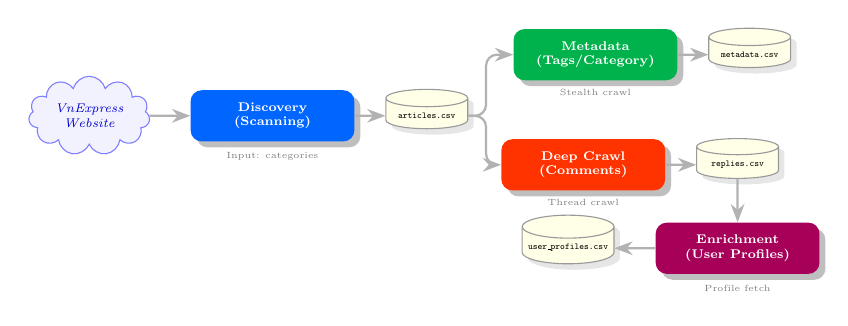
\begin{tikzpicture}[
            scale=0.65, transform shape,
            node distance=0.6cm and 0.9cm,
            process/.style={
                    rectangle, rounded corners=4pt,
                    minimum width=3.2cm, minimum height=1.0cm,
                    align=center, text=white,
                    font=\scriptsize\bfseries, drop shadow
                },
            step1/.style={process, fill=blue!60!cyan},
            step2/.style={process, fill=red!60!orange},
            step3/.style={process, fill=purple!60!violet},
            step4/.style={process, fill=teal!60!green},
            data/.style={
                    cylinder, shape border rotate=90,
                    draw=gray!80, fill=yellow!10, aspect=0.25,
                    minimum height=0.75cm, minimum width=1.6cm,
                    align=center, font=\tiny\ttfamily,
                    drop shadow={opacity=0.2}
                },
            source/.style={
                    cloud, cloud puffs=11,
                    draw=blue!50, fill=blue!5, aspect=2,
                    minimum width=2.0cm, minimum height=1.2cm,
                    align=center, font=\scriptsize\itshape\color{blue!80!black}
                },
            arrow/.style={-Stealth, thick, draw=gray!60, rounded corners}
        ]
        \node[source] (web) {VnExpress\\Website};

        \node[step1, right=0.8cm of web] (s1) {Discovery\\(Scanning)};
        \node[data, right=0.6cm of s1] (d1) {articles.csv};

        \node[step4, above right=0.2cm and 1.2cm of d1] (s4) {Metadata\\(Tags/Category)};
        \node[data, right=0.6cm of s4] (d4) {metadata.csv};

        \node[step2, below right=0.2cm and 1.2cm of d1] (s2) {Deep Crawl\\(Comments)};
        \node[data, right=0.6cm of s2] (d2) {replies.csv};

        \node[step3, below=0.85cm of d2] (s3) {Enrichment\\(User Profiles)};
        \node[data, left=0.8cm of s3] (d3) {user\_profiles.csv};

        \draw[arrow] (web) -- (s1);
        \draw[arrow] (s1) -- (d1);
        \draw[arrow] (d1.east) -- ++(0.35,0) |- (s4.west);
        \draw[arrow] (d1.east) -- ++(0.35,0) |- (s2.west);
        \draw[arrow] (s4) -- (d4);
        \draw[arrow] (s2) -- (d2);
        \draw[arrow] (d2.south) -- (s3.north);
        \draw[arrow] (s3) -- (d3);

        \node[text=gray, font=\tiny, align=center, below=0.08cm of s1] {Input: categories};
        \node[text=gray, font=\tiny, align=center, below=0.05cm of s4] {Stealth crawl};
        \node[text=gray, font=\tiny, align=center, below=0.05cm of s2] {Thread crawl};
        \node[text=gray, font=\tiny, align=center, below=0.1cm of s3] {Profile fetch};
    \end{tikzpicture}
    \caption{Data crawling pipeline and intermediate tables for graph construction.}
    \label{fig:crawler-pipeline}
\end{figure*}

\subsection{Data schema}
\autoref{tab:schema} summarizes the schema of normalized tables,
used as input for graph construction and model training.

\begin{table}[t]
    \centering
    \small
    \setlength{\tabcolsep}{4pt}
    \begin{tabular}{l p{5.6cm}}
        \toprule
        \textbf{Table} & \textbf{Main fields}                                                                     \\
        \midrule
        Articles       & \texttt{article\_id, url, title, short\_description, author, published\_at, content}     \\
        Metadata       & \texttt{article\_url, category, tags}                                                    \\
        Replies        & \texttt{article\_url, parent\_user\_id, parent\_text, ..., reply\_user\_id, reply\_text} \\
        User Profiles  & \texttt{user\_id, username, join\_date}                                                  \\
        \bottomrule
    \end{tabular}
    \caption{Summary of the normalized data schema.}
    \label{tab:schema}
\end{table}

\subsection{Summary statistics and sparsity}
After crawling and cleaning, the dataset contains \textbf{3,645} articles, \textbf{15,693} users, and \textbf{40,045} interactions (comments/replies).
On average, each user has only \textbf{2.55} interactions, and each article has about \textbf{10.99} interactions.

Sparsity of the user--article interaction matrix is computed as:
\begin{equation}
    \text{Sparsity} = 1 - \frac{40{,}045}{15{,}693 \times 3{,}645} \approx 99.93\%.
    \label{eq:sparsity}
\end{equation}
This extremely high sparsity indicates severe cold-start risk,
because most users and articles provide very limited direct interaction signals,
making purely collaborative filtering difficult.

\subsection{Article category distribution}
\autoref{fig:eda-category} shows that the number of articles across categories is relatively balanced.
This helps reduce bias in article counts,
but it does not guarantee uniform engagement,
since commenting behavior strongly depends on the topic.
Therefore, later analyses focus on interaction and degree distributions
to better characterize sparsity and user behavior.

\begin{figure}[t]
    \centering
    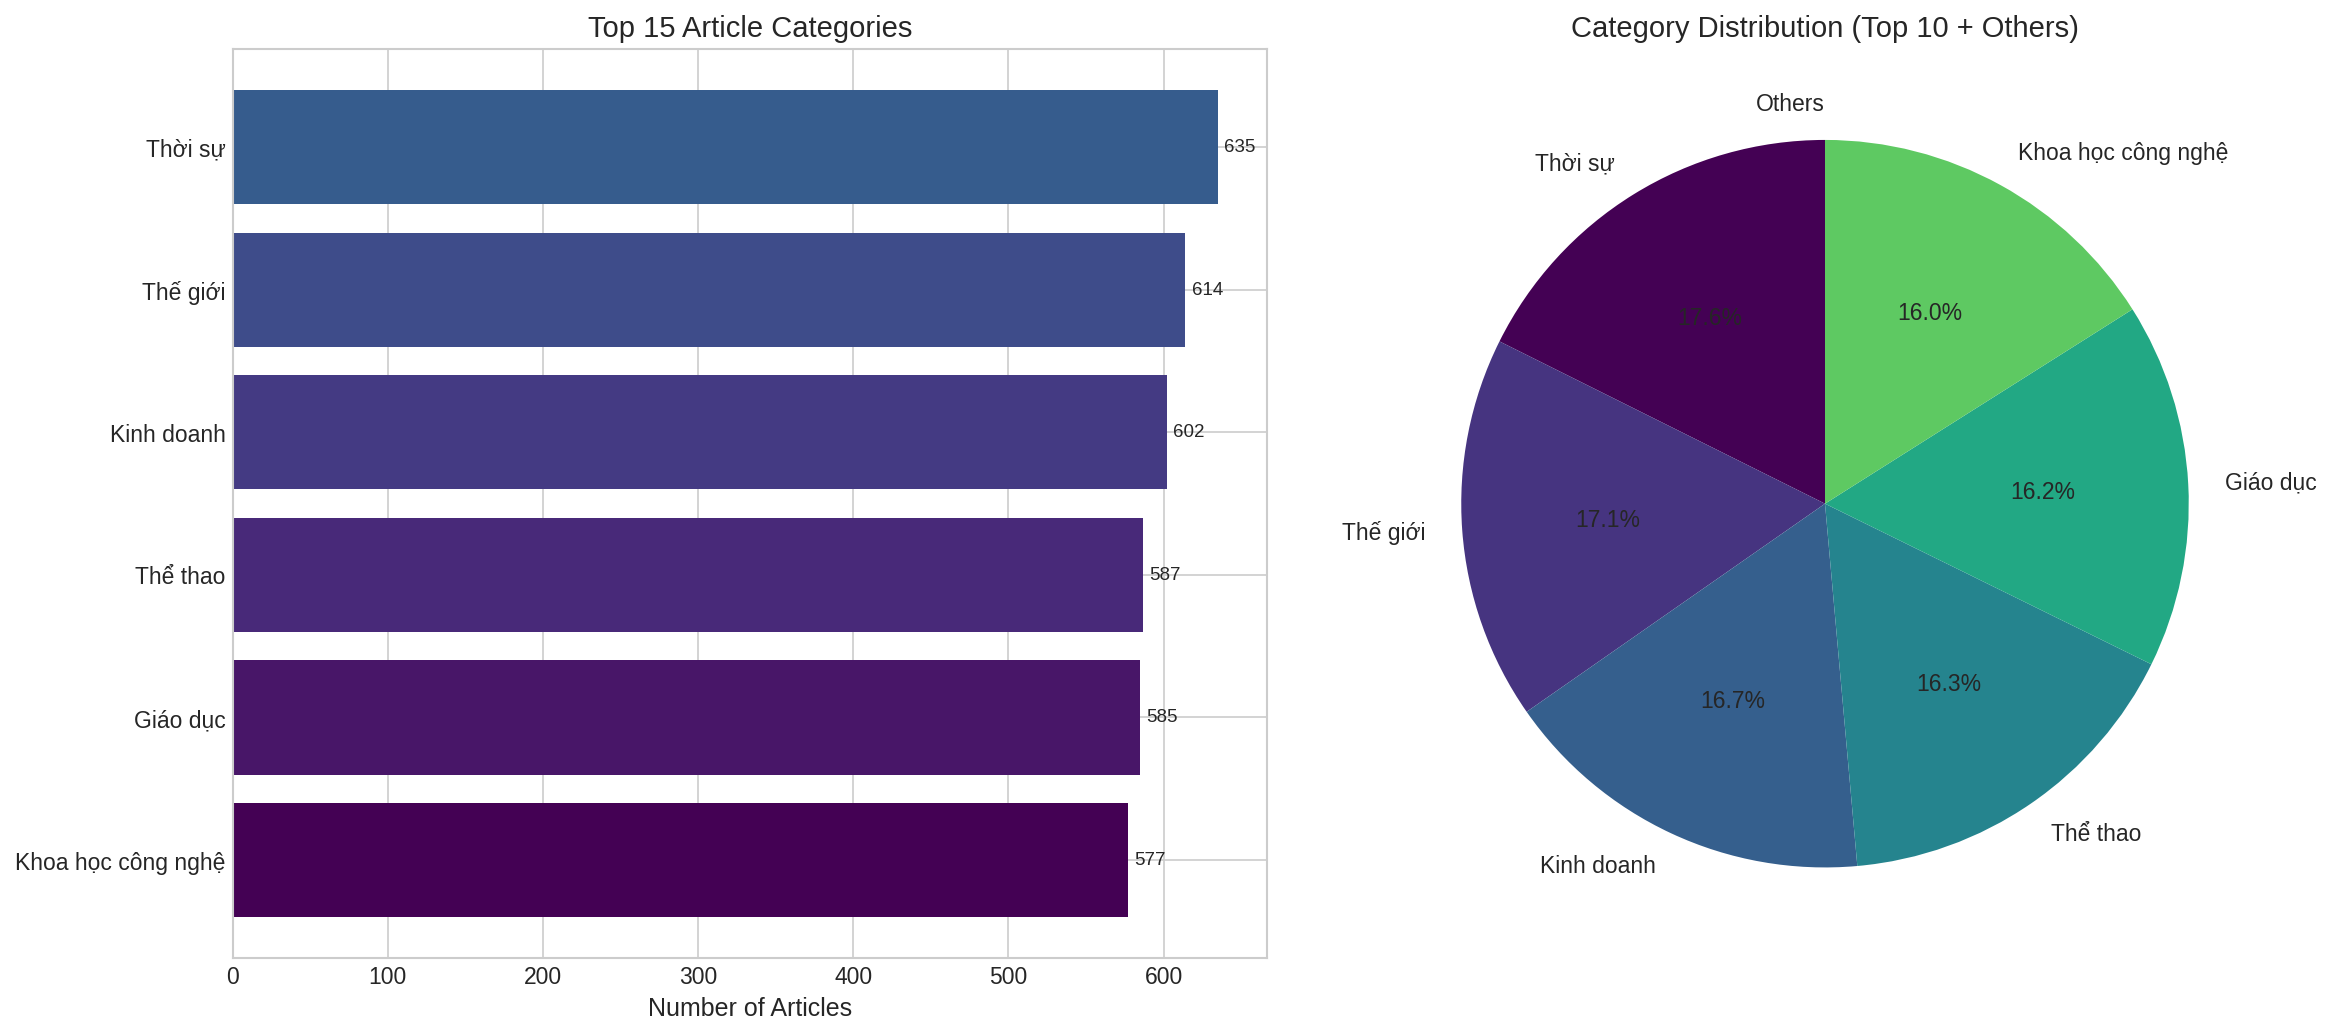
\includegraphics[width=\linewidth]{eda_09_metadata_categories.png}
    \caption{Distribution of articles by category.}
    \label{fig:eda-category}
\end{figure}

\subsection{User activity and long-tail behavior}
\autoref{fig:eda-user-bottom} illustrates a power-law activity distribution:
a small group of users contributes most interactions,
while the majority produces only a few comments (long-tail).
This leads to two key consequences:
(i) embeddings for low-activity users are difficult to learn stably,
and (ii) a small number of high-degree users can become hubs,
dominating message passing.
Thus, relying only on user--article interactions (G1)
is limited under extreme sparsity,
motivating the addition of social user--user edges (G2)
to enable indirect information propagation.

\begin{figure}[t]
    \centering
    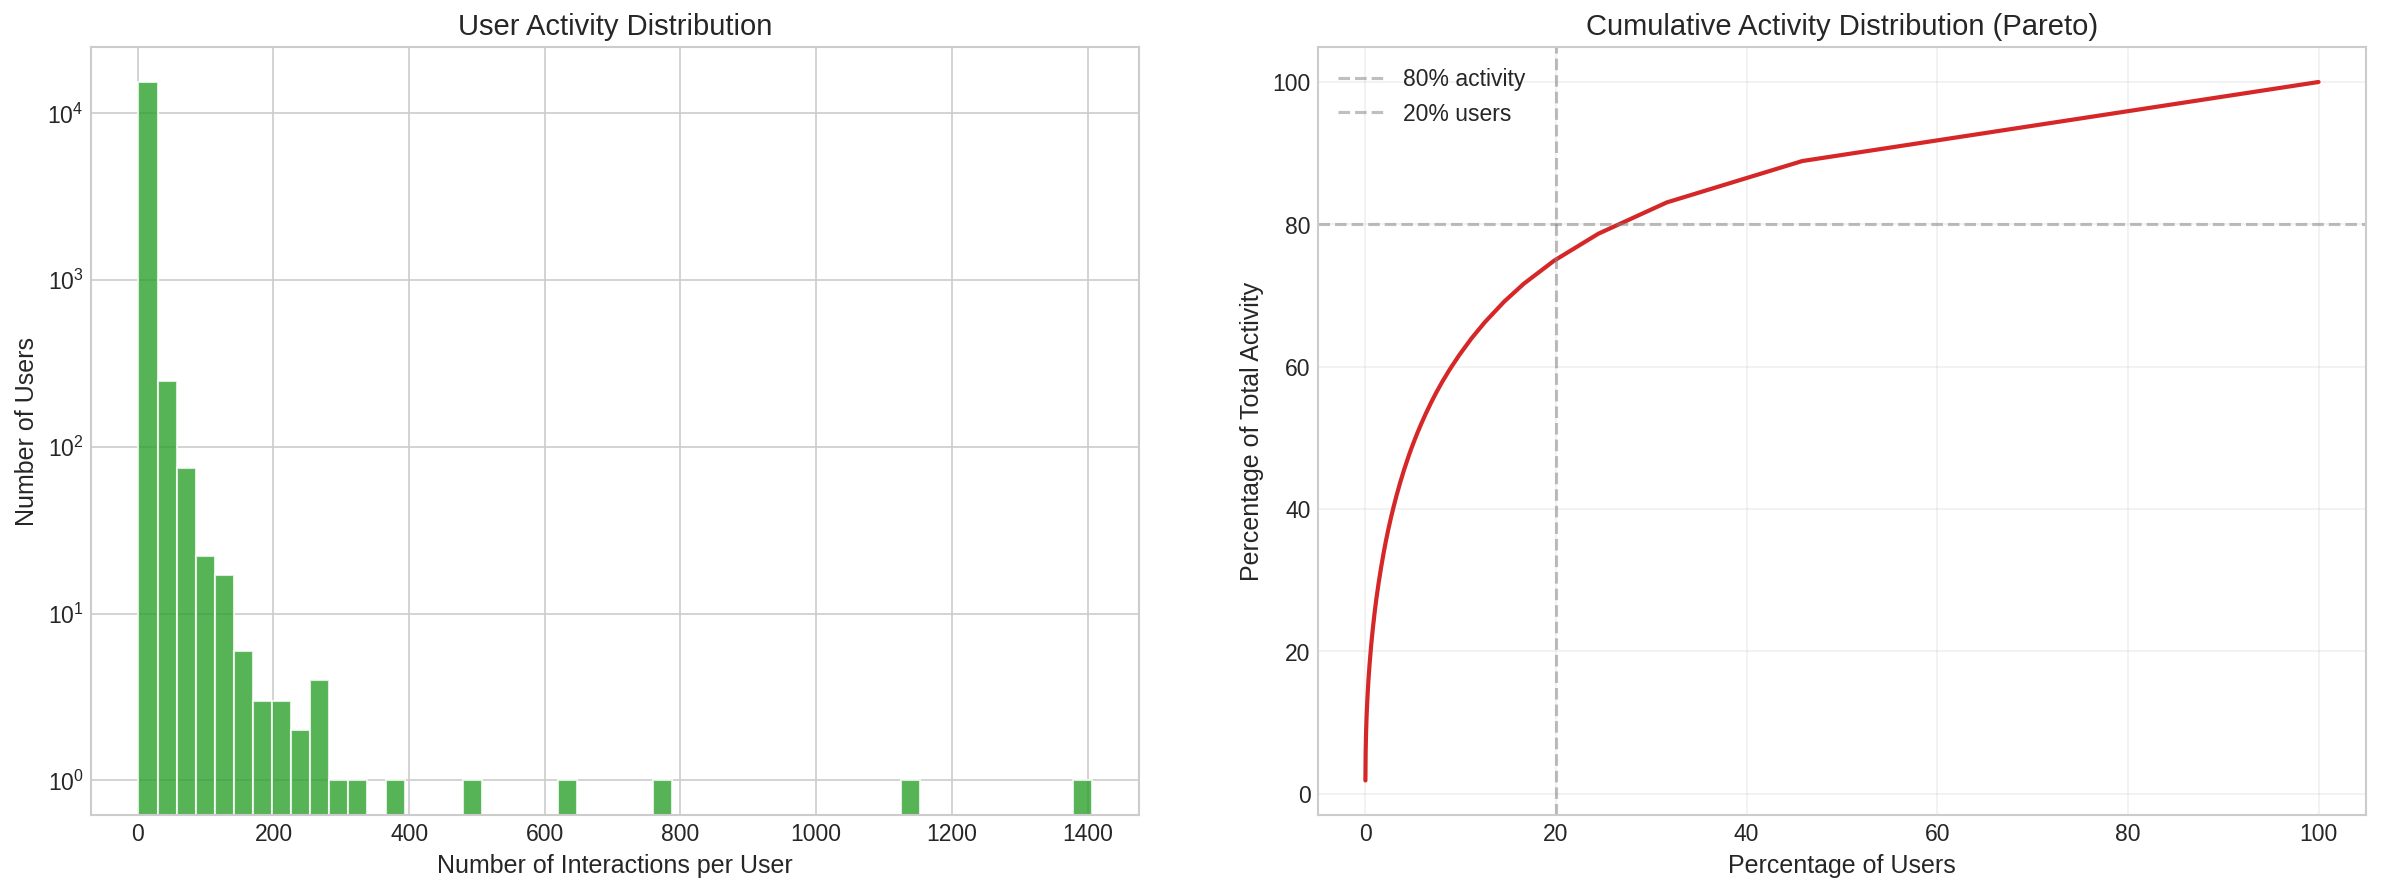
\includegraphics[width=\linewidth]{eda_03_user_activity_bottom.png}
    \caption{User activity exhibits a power-law trend.}
    \label{fig:eda-user-bottom}
\end{figure}

\subsection{Engagement by category}
\autoref{fig:eda-eng-by-cat} shows significant differences in
the total number of comments and the average comments per article across categories.
Some categories are more discussion-intensive,
while others receive less engagement.
This suggests that category is a coarse semantic signal,
but it does not represent uniform interaction behavior.
Therefore, adding \textit{category nodes} (G3)
may shorten paths in the graph,
but it can also risk over-generalization
when high-degree category hubs pull embeddings toward generic features,
reducing personalization.

\begin{figure}[t]
    \centering
    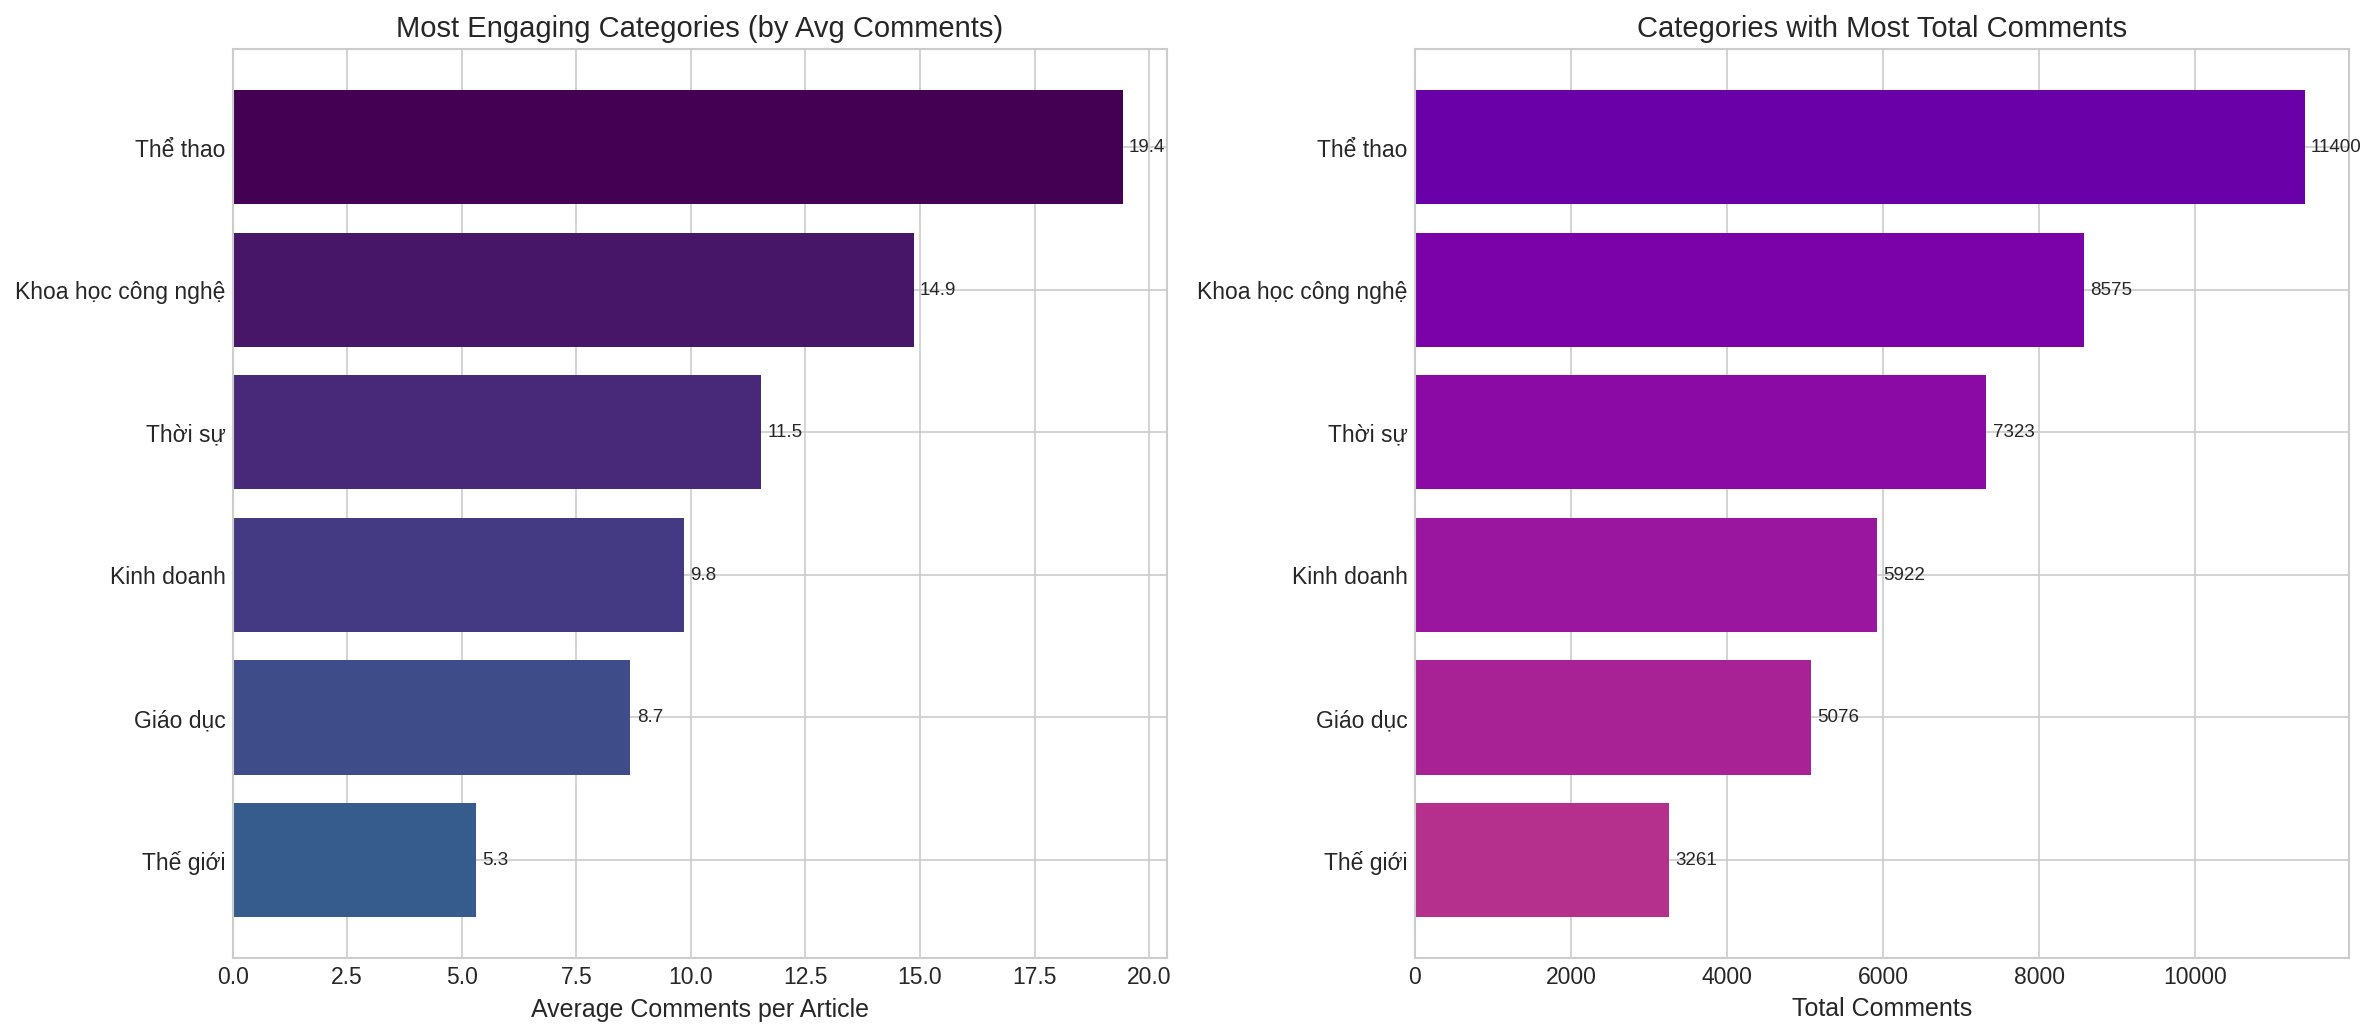
\includegraphics[width=\linewidth]{eda_11_engagement_by_category.png}
    \caption{Engagement by category.}
    \label{fig:eda-eng-by-cat}
\end{figure}

\subsection{Degree distribution and implications for graph learning}
\autoref{fig:degree} presents the degree distributions of users and articles in the interaction graph.
On the user side, most users have very small degrees,
reflecting high cold-start risk.
On the article side, most articles receive only a few comments,
while a small number of ``hot'' articles have high degrees,
consistent with the time-sensitive and short-lived nature of news.
These skewed distributions challenge signal propagation:
low-degree nodes lack sufficient signals to learn representations,
while high-degree nodes increase the risk of over-smoothing as depth increases.
These observations support evaluating multiple graph structures (G1--G3)
and models with embedding-stabilization mechanisms such as graph contrastive learning.

\begin{figure}[t]
    \centering
    \begin{subfigure}{.49\linewidth}
        \centering
        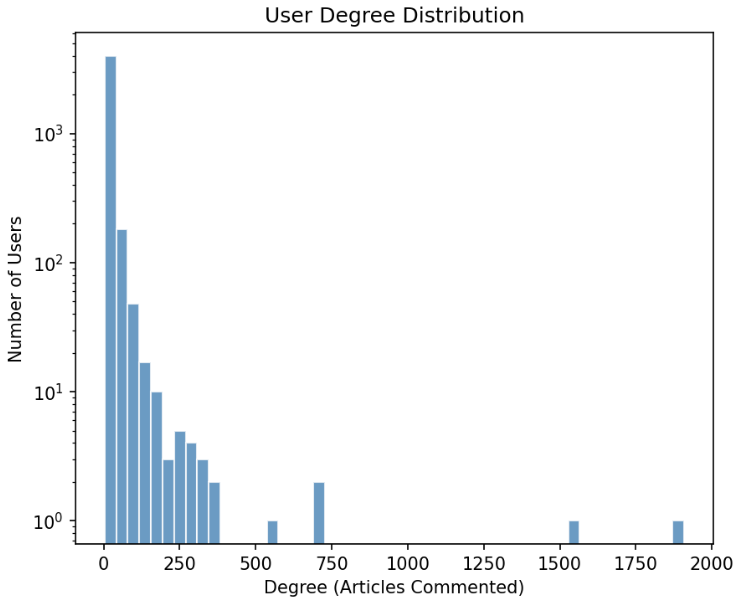
\includegraphics[width=\linewidth]{users_dis.png}
        \caption{Users}
    \end{subfigure}
    \begin{subfigure}{.49\linewidth}
        \centering
        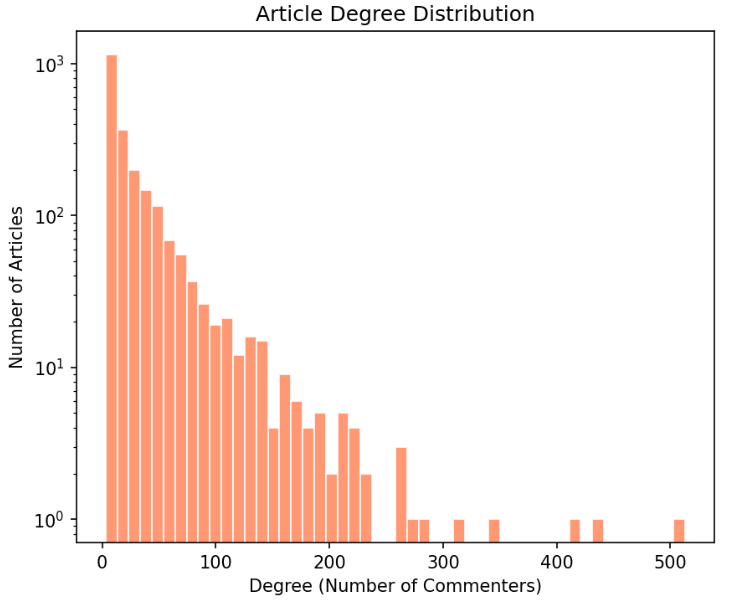
\includegraphics[width=\linewidth]{articles_dis.png}
        \caption{Articles}
    \end{subfigure}
    \caption{Degree distributions in the interaction graph.}
    \label{fig:degree}
\end{figure}

\textbf{Summary.}
Overall, the EDA shows that the VnExpress data is extremely sparse,
strongly long-tailed for both users and articles,
and exhibits notable differences in engagement across categories.
These characteristics explain the limitations of purely collaborative filtering
and motivate enriching graph signals via indirect links
and controlling propagation in heterogeneous graphs.

% ==========================================================
\section{Graph Design and Expansion Strategy (G1--G3)}
\label{sec:graph}

\subsection{Overall idea}
With very high sparsity \eqref{eq:sparsity}, a pure user--article graph struggles to propagate signals for low-activity users. Therefore, we design three graph structures with increasing richness:
\begin{itemize}
    \item \textbf{G1 (Bipartite):} only users and articles with interaction edges.
    \item \textbf{G2 (Social expansion):} adds user--user edges derived from replies in discussions.
    \item \textbf{G3 (Category hubs):} adds category nodes to shorten paths between users and groups of articles in the same category.
\end{itemize}

\subsection{Node/edge definitions and graph construction}
We denote a graph as $\mathcal{G}=(\mathcal{V},\mathcal{E})$ with node sets: users ($U$), articles ($A$), and categories ($C$). Observed interactions come from \textit{comments/replies}, thus we treat them as \textbf{implicit feedback}.

\textbf{User--article edges.} An edge $(u,a)\in \mathcal{E}_{u-a}$ is created if user $u$ has at least one comment under article $a$. In the basic setting, edges are treated as \textbf{undirected} and \textbf{unweighted} to isolate the effect of graph structure. This keeps experimental settings consistent across compared models and separates structural effects from edge weighting effects.

\textbf{User--user edges (social links).} From the discussion structure, if $u_i$ replies to $u_j$, we create an edge $(u_i,u_j)\in \mathcal{E}_{u-u}$. Since the goal is to propagate preference signals within discussion communities, we \textbf{symmetrize} these edges to reflect \textit{social homophily} rather than a one-way causal relation.

\subsection{Three graph variants and design intuition}
\label{sec:graph_configs}

Based on EDA, we design three graph variants $\mathcal{G}_1, \mathcal{G}_2, \mathcal{G}_3$ with increasing complexity to evaluate the impact of each structural signal type.

\textbf{G1: Basic bipartite graph.}
This is the standard configuration for collaborative filtering graph models. The graph contains only users $U$ and articles $A$, with edges $\mathcal{E}_{u-a}$ representing comment interactions.
\begin{itemize}
    \item \textbf{Structure:} a bipartite (two-part) graph.
    \item \textbf{Intuition:} captures direct preferences. However, with sparsity of $99.93\%$, the graph contains many disconnected components, limiting message passing for long-tail users.
\end{itemize}

\textbf{G2: Graph with social expansion.}
To reduce the information fragmentation in G1, we expand the graph by incorporating user--user relations, turning it into a heterogeneous multi-relation graph. Specifically, G2 adds two types of user--user edges:
\begin{itemize}
    \item \textbf{Explicit Social (Reply):} An edge $(u_i, u_j)$ if $u_i$ replies to $u_j$. This captures direct social interaction in discussions.
    \item \textbf{Implicit Homophily (Shared Interest):} An edge $(u_i, u_j)$ if two users interact with at least $k$ common articles (in our experiments, $k=2$). This captures latent shared interests even without direct replies.
\end{itemize}
\textbf{Intuition:} Adding lateral ($u-u$) edges creates ``bridges'' for embedding propagation among users, enriching representations even when user--article interactions are extremely sparse.

\textbf{G3: Semantic category graph.}
G3 tackles sparsity from a content perspective. We add category nodes $C$ and two new edge types:
\begin{itemize}
    \item \textbf{Article--Category:} a deterministic attribute relation from metadata (e.g., article $a$ belongs to \textit{Sports}).
    \item \textbf{User--Category:} a preference relation aggregated from interaction history (edge weight proportional to how many articles in a category the user commented on).
\end{itemize}
\textbf{Intuition:} Category nodes act as ``semantic hubs''. They create short length-2 paths ($u \to c \to a'$) that connect users to new articles in the same category even with limited interactions, but they can also introduce high-degree hubs that may cause noise.

\subsection{Illustration of G1--G3}
\autoref{fig:g123} shows that moving from G1 to G2 connects users via social edges, improving embedding propagation among users with similar discussion behavior. In G3, category hubs create short paths between users and groups of articles in the same category, but can also introduce overly high-degree nodes that may increase noise.

\begin{figure*}[!t]
    \centering
    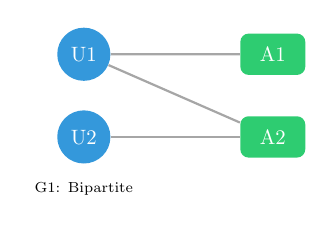
\begin{tikzpicture}[scale=0.75, transform shape]
        \node[circle, fill=userblue, text=white, minimum size=0.9cm] (u1) at (0,1.4) {U1};
        \node[circle, fill=userblue, text=white, minimum size=0.9cm] (u2) at (0,0) {U2};
        \node[rectangle, rounded corners=3pt, fill=articlegreen, text=white, minimum width=1.1cm, minimum height=0.7cm] (a1) at (3.2,1.4) {A1};
        \node[rectangle, rounded corners=3pt, fill=articlegreen, text=white, minimum width=1.1cm, minimum height=0.7cm] (a2) at (3.2,0) {A2};
        \draw[-, thick, gray!70] (u1)--(a1);
        \draw[-, thick, gray!70] (u1)--(a2);
        \draw[-, thick, gray!70] (u2)--(a2);
        \node[below=0.2cm of u2, font=\scriptsize] {G1: Bipartite};
    \end{tikzpicture}
    \hspace{0.5cm}
    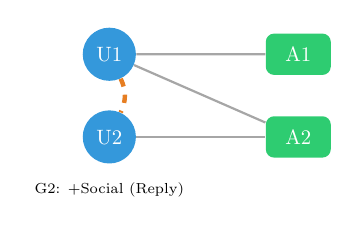
\begin{tikzpicture}[scale=0.75, transform shape]
        \node[circle, fill=userblue, text=white, minimum size=0.9cm] (u1) at (0,1.4) {U1};
        \node[circle, fill=userblue, text=white, minimum size=0.9cm] (u2) at (0,0) {U2};
        \node[rectangle, rounded corners=3pt, fill=articlegreen, text=white, minimum width=1.1cm, minimum height=0.7cm] (a1) at (3.2,1.4) {A1};
        \node[rectangle, rounded corners=3pt, fill=articlegreen, text=white, minimum width=1.1cm, minimum height=0.7cm] (a2) at (3.2,0) {A2};
        \draw[-, thick, gray!70] (u1)--(a1);
        \draw[-, thick, gray!70] (u1)--(a2);
        \draw[-, thick, gray!70] (u2)--(a2);
        \draw[-, dashed, ultra thick, socialorange, bend left=25] (u1) to (u2);
        \node[below=0.2cm of u2, font=\scriptsize] {G2: +Social (Reply)};
    \end{tikzpicture}
    \hspace{0.5cm}
    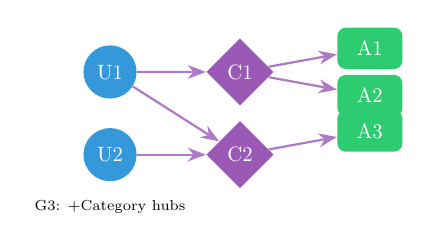
\begin{tikzpicture}[scale=0.75, transform shape]
        \node[circle, fill=userblue, text=white, minimum size=0.9cm] (u1) at (0,1.4) {U1};
        \node[circle, fill=userblue, text=white, minimum size=0.9cm] (u2) at (0,0) {U2};
        \node[diamond, fill=cathub, text=white, minimum size=1.0cm] (c1) at (2.2,1.4) {C1};
        \node[diamond, fill=cathub, text=white, minimum size=1.0cm] (c2) at (2.2,0) {C2};
        \node[rectangle, rounded corners=3pt, fill=articlegreen, text=white, minimum width=1.1cm, minimum height=0.7cm] (a1) at (4.4,1.8) {A1};
        \node[rectangle, rounded corners=3pt, fill=articlegreen, text=white, minimum width=1.1cm, minimum height=0.7cm] (a2) at (4.4,1.0) {A2};
        \node[rectangle, rounded corners=3pt, fill=articlegreen, text=white, minimum width=1.1cm, minimum height=0.7cm] (a3) at (4.4,0.4) {A3};
        \draw[-Stealth, thick, cathub!80] (u1)--(c1);
        \draw[-Stealth, thick, cathub!80] (u1)--(c2);
        \draw[-Stealth, thick, cathub!80] (u2)--(c2);
        \draw[-Stealth, thick, cathub!80] (c1)--(a1);
        \draw[-Stealth, thick, cathub!80] (c1)--(a2);
        \draw[-Stealth, thick, cathub!80] (c2)--(a3);
        \node[below=0.2cm of u2, font=\scriptsize] {G3: +Category hubs};
    \end{tikzpicture}
    \caption{Illustration of the three graph layers G1--G3.}
    \label{fig:g123}
\end{figure*}

\subsection{Temporal splitting to reduce leakage}
For news data, interactions are strongly time-dependent. When building train/test sets, ensuring that training comes from the past and testing comes from the future better simulates deployment \cite{wang2023leakage}. In our experiments, we use a \textbf{chronological split}: earlier interactions are used for training and later interactions for testing, with a split time $T_{\text{split}}$ as shown in \autoref{fig:temporal-split}. This prevents the model from observing future information during training.

\begin{figure}[t]
    \centering
    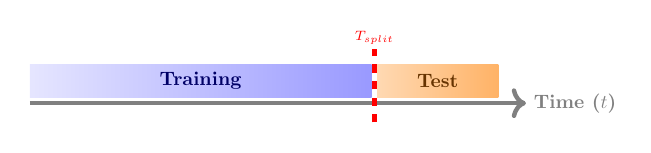
\begin{tikzpicture}[scale=0.7, transform shape]
        \draw[->, ultra thick, gray] (0,0) -- (9,0) node[right, font=\bfseries] {Time ($t$)};
        \shade[left color=blue!10, right color=blue!40] (0,0.1) rectangle (6.2,0.7);
        \node[blue!40!black] at (3.1, 0.4) {\textbf{Training}};
        \shade[left color=orange!30, right color=orange!60] (6.3,0.1) rectangle (8.5,0.7);
        \node[orange!40!black] at (7.4, 0.4) {\textbf{Test}};
        \draw[dashed, red, ultra thick] (6.25, -0.35) -- (6.25, 1.05);
        \node[red, font=\bfseries\scriptsize, fill=white, inner sep=2pt] at (6.25, 1.18) {$T_{split}$};
    \end{tikzpicture}
    \caption{Illustration of a temporal train/test split.}
    \label{fig:temporal-split}
\end{figure}

% ==========================================================
\section{Method}
\label{sec:method}

\subsection{Problem definition and notation}
Let $U$ be the set of users and $A$ be the set of articles.
Observed interactions come from commenting and replying,
thus we treat this as an implicit-feedback recommendation problem.
The goal is to learn a scoring function $f(u,a)$
that estimates the compatibility between user $u \in U$ and article $a \in A$,
then rank and recommend Top-$K$ articles that $u$ has not interacted with.

In graph-based models,
each user and article is represented by an embedding in a latent space.
The relevance score $f(u,a)$ is computed as the dot product between user and article embeddings,
consistent with the standard setup in graph collaborative filtering.

\subsection{Content-based baselines}
To evaluate the role of structural signals versus content,
we compare with strong content-based methods that rely only on article text:
\begin{itemize}
    \item \textbf{TF-IDF:} A traditional keyword-frequency method,
          representing text as sparse vectors and measuring similarity by cosine similarity.
    \item \textbf{PhoBERT:} A state-of-the-art Vietnamese pre-trained language model,
          used to extract dense semantic embeddings from titles and descriptions.
    \item \textbf{VnDoc} (\texttt{dangvantuan/vietnamese-document-embedding}): A Vietnamese document embedding model
          optimized for classification and search tasks.
    \item \textbf{BGE-M3:} A modern multilingual embedding model
          that supports multi-vector representations and performs strongly across benchmarks, including Vietnamese.
\end{itemize}
These methods serve as strong baselines in cold-start settings,
where historical interaction signals are limited.

\subsection{Graph baselines}
\textbf{LightGCN.}
LightGCN is a widely used baseline for recommendation on bipartite user--item graphs,
thanks to a simplified GCN design.
It removes nonlinearities and learnable transformations between layers,
keeping only linear propagation through the normalized adjacency matrix:
\[
    \mathbf{E}^{(k)} = \hat{\mathbf{A}} \mathbf{E}^{(k-1)}, \quad
    \mathbf{E}^{*}=\sum_{k=0}^{K}\alpha_k \mathbf{E}^{(k)}.
\]
This design makes LightGCN both effective and stable in many recommendation tasks.

\textbf{SimGCL, XSimGCL, and LightGCL.}
These models extend LightGCN by adding contrastive learning
to improve embedding robustness under sparse data.
SimGCL perturbs embeddings during propagation.
XSimGCL further simplifies the contrastive design to reduce training cost
while retaining effectiveness.
LightGCL adds a global-context component
to compensate for limitations of learning only from local neighborhoods via an SVD-based view.

\subsection{HGN: Multi-Aspect Heterogeneous GNN}
VnExpress news data contains multiple relation types, notably:
(i) \textit{user--article} interactions (commenting) reflecting content preferences, and
(ii) \textit{user--user} relations (replying) reflecting \textit{social homophily}.
To jointly model these signals while preserving relation semantics, we propose \textbf{HGN} based on \textbf{Heterogeneous Graph Convolution} (HeteroConv).

Unlike traditional GNNs that treat all edges equally, HGN performs relation-aware message passing.
At layer $l$, the embedding of user $u$ is updated by aggregating information from all neighborhoods, using relation-specific transformations:
\begin{equation}
    \mathbf{h}_u^{(l+1)} = \sigma \left( \sum_{r \in \mathcal{R}} \text{CONV}_r \left( \mathbf{h}_u^{(l)}, \{ \mathbf{h}_v^{(l)} \mid v \in \mathcal{N}_u^r \} \right) \right)
    \label{eq:hetero_agg}
\end{equation}
where:
\begin{itemize}
    \item $\mathcal{R}$ is the set of relations, including \textit{comments} (article interactions), \textit{replied\_to} (direct social interactions), and \textit{interacts\_with} (implicit social homophily).
    \item $\text{CONV}_r$ is a relation-specific GNN module. In our experiments, we use \textbf{TransformerConv} to leverage multi-head attention, allowing the model to weight the importance of different neighbors automatically.
\end{itemize}
This aggregation mechanism enables HGN to softly integrate social signals into preference signals during learning, producing embeddings that are richer and more robust under extreme sparsity.

\subsection{HCL: Exploring Heterogeneous Contrastive Learning}
HCL is designed as a counterfactual method that combines a dual-path architecture with the SimGCL-style idea of contrastive learning to enhance representational discrimination. Instead of immediately mixing signals as in HGN, HCL separates propagation into two independent streams to preserve each aspect:
\begin{itemize}
    \item \textbf{Interest view:} propagate embeddings on the bipartite graph $\mathcal{G}_{u-a}$ using \textbf{LightGCN} for computational efficiency.
    \item \textbf{Social view:} propagate embeddings on the social graph $\mathcal{G}_{u-u}$ to capture community structure.
\end{itemize}

The two streams are then fused via learnable weighted fusion:
\begin{equation}
    \mathbf{h}_u^{final} = w_{int} \cdot \mathbf{h}_u^{int} + w_{soc} \cdot \mathbf{h}_u^{soc}
\end{equation}
where $w_{int}$ and $w_{soc}$ are learnable parameters. HCL optimizes a multi-task objective combining BPR Loss and Contrastive Loss:
\begin{equation}
    \mathcal{L} = \mathcal{L}_{BPR} + \lambda \cdot \mathcal{L}_{InfoNCE} + \gamma \cdot \mathcal{L}_{Reg}
\end{equation}
where $\mathcal{L}_{InfoNCE}$ matches views produced by adding random noise perturbations to embeddings. However, experiments show that HCL is sensitive to hyperparameters under VnExpress extreme sparsity, so HGN remains our primary proposed model.

\section{Experimental Setup}
\label{sec:exp}

\subsection{Training setup}
All models are trained for 100 epochs
with batch size 2048.
Graph-based models are optimized with Adam
with learning rate $10^{-3}$ and embedding dimension 64.
The main recommendation loss is BPR loss,
consistent with implicit-feedback settings.
For models with contrastive learning,
an InfoNCE loss is added and combined with BPR.

During training,
negative samples are randomly drawn from articles
that the user has not interacted with.
Hyperparameters are kept consistent across models
to ensure fair comparison.

\subsection{Evaluation protocols}
Because news data is strongly time-dependent, we use two evaluation protocols
to better reflect deployment settings.

\textbf{Full Ranking (Global).}
Interactions are sorted by time and split 80/20 (chronological split),
where past interactions are used for training and future interactions for testing.
This setting evaluates a model's ability to predict user behavior in realistic news recommendation.

\textbf{Leave-One-Out (Loo100).}
For each user, the latest interaction is kept as the positive sample,
combined with 99 unseen articles as negative samples.
This protocol evaluates local ranking quality
when the candidate set is narrowed.

\subsection{Evaluation metrics}
We evaluate model performance using standard recommendation metrics:
\begin{itemize}
    \item \textbf{Recall@10}: Measures coverage,
          reflecting whether the correct item appears in the top-10 list.
    \item \textbf{Hit Rate@10 (HR)}: Measures basic user experience,
          checking whether the top-10 contains at least one relevant article.
    \item \textbf{NDCG@10}: Measures ranking quality,
          rewarding models that place relevant items higher.
    \item \textbf{MRR}: Suitable for news recommendation,
          measuring how quickly the system returns the first relevant result.
\end{itemize}

% ==========================================================
\section{Results and Analysis}
\label{sec:results}

\subsection{Full Ranking results}
\autoref{tab:results_full} summarizes results by graph variant. Under cold-start, content-based models show clear advantages because they match deep semantic similarity from text and depend less on graph sparsity. This indicates that for global retrieval in a large search space, article content is the most reliable signal. In contrast, for graph-based models, expanding to G2 (adding social edges) improves propagation compared to G1, but still suffers due to sparsity. This is consistent with EDA: most users and articles have very few interactions, making structural signals hard to leverage in a large candidate space.

\begin{table}[!htbp]
    \centering
    \scriptsize
    \setlength{\tabcolsep}{1.5pt}
    \renewcommand{\arraystretch}{1.1}
    \rowcolors{2}{gray!5}{white}
    \caption{Full Ranking results (ranking over the full candidate set of over 3{,}600 articles). Best results are in \textbf{bold}.}
    \label{tab:results_full}
    \begin{tabularx}{\linewidth}{l|c|*4{>{\centering\arraybackslash}X}}
        \toprule
        \textbf{Model} & \textbf{Type} & \textbf{R@10}   & \textbf{N@10}   & \textbf{H@10}   & \textbf{MRR}    \\
        \midrule
        \multicolumn{6}{l}{\textit{\textbf{Content-Based / Baselines}}}                                        \\
        BGE-M3         & CB            & \textbf{0.0535} & \textbf{0.0315} & \textbf{0.0929} & \textbf{0.0416} \\
        TF-IDF         & CB            & 0.0508          & 0.0301          & 0.0951          & 0.0394          \\
        VnDoc          & CB            & 0.0485          & 0.0287          & 0.0832          & 0.0362          \\
        PhoBERT        & CB            & 0.0452          & 0.0253          & 0.0850          & 0.0335          \\
        \midrule
        \multicolumn{6}{l}{\textit{\textbf{Graph G1 (Bipartite)}}}                                             \\
        LightGCL       & G-CL          & 0.0398          & 0.0249          & 0.0685          & 0.0313          \\
        LightGCN       & G-GNN         & 0.0263          & 0.0145          & 0.0400          & 0.0174          \\
        XSimGCL        & G-CL          & \textbf{0.0439} & \textbf{0.0253} & \textbf{0.0694} & \textbf{0.0289} \\
        HGN            & H-GNN         & 0.0262          & 0.0147          & 0.0451          & 0.0182          \\
        HCL            & H-CL          & 0.0259          & 0.0164          & 0.0471          & 0.0214          \\
        SimGCL         & G-CL          & 0.0191          & 0.0115          & 0.0275          & 0.0135          \\
        \midrule
        \multicolumn{6}{l}{\textit{\textbf{Graph G2 (User--User Social)}}}                                     \\
        LightGCL       & G-CL          & \textbf{0.0436} & \textbf{0.0261} & \textbf{0.0739} & \textbf{0.0313} \\
        LightGCN       & G-GNN         & 0.0272          & 0.0156          & 0.0404          & 0.0186          \\
        XSimGCL        & G-CL          & 0.0432          & 0.0260          & 0.0688          & 0.0303          \\
        HGN (Ours)     & H-GNN         & 0.0369          & 0.0201          & 0.0596          & 0.0250          \\
        HCL (Ours)     & H-CL          & 0.0320          & 0.0192          & 0.0520          & 0.0233          \\
        SimGCL         & G-CL          & 0.0228          & 0.0131          & 0.0312          & 0.0144          \\
        \midrule
        \multicolumn{6}{l}{\textit{\textbf{Graph G3 (Category Hubs)}}}                                         \\
        LightGCL       & G-CL          & \textbf{0.0413} & \textbf{0.0256} & \textbf{0.0710} & \textbf{0.0311} \\
        LightGCN       & G-GNN         & 0.0258          & 0.0145          & 0.0388          & 0.0175          \\
        XSimGCL        & G-CL          & 0.0379          & 0.0232          & 0.0643          & 0.0289          \\
        HGN (Ours)     & H-GNN         & 0.0299          & 0.0167          & 0.0464          & 0.0198          \\
        HCL (Ours)     & H-CL          & 0.0250          & 0.0152          & 0.0471          & 0.0205          \\
        SimGCL         & G-CL          & 0.0222          & 0.0122          & 0.0322          & 0.0137          \\
        \bottomrule
    \end{tabularx}
\end{table}

\subsection{Loo100 results}
Under Loo100, HGN on G2 achieves the best performance, showing a reversal compared to Full Ranking. We argue that in a narrow candidate space (Local Discrimination), subtle structural signals (such as social links in G2) become more discriminative than pure content, helping separate the target positive item from random negatives. This phenomenon has also been reported in prior work: evaluation on small candidate sets highlights structural signals more than pure content.

\begin{table}[!htbp]
    \centering
    \scriptsize
    \setlength{\tabcolsep}{1.5pt}
    \renewcommand{\arraystretch}{1.1}
    \rowcolors{2}{gray!5}{white}
    \caption{Leave-One-Out (Loo100) results for the three graph structures.}
    \label{tab:loo100}
    \begin{tabularx}{\linewidth}{l|c|*4{>{\centering\arraybackslash}X}}
        \toprule
        \textbf{Model} & \textbf{Type} & \textbf{R@10}   & \textbf{N@10}   & \textbf{H@10}   & \textbf{MRR}    \\
        \midrule
        \multicolumn{6}{l}{\textit{\textbf{Graph G1 (Bipartite)}}}                                             \\
        LightGCL       & G-CL          & \textbf{0.3081} & \textbf{0.2021} & \textbf{0.3822} & \textbf{0.2060} \\
        LightGCN       & G-GNN         & 0.2818          & 0.1743          & 0.3595          & 0.1782          \\
        XSimGCL        & G-CL          & 0.3009          & 0.1972          & 0.3787          & 0.2063          \\
        HGN            & H-GNN         & 0.2740          & 0.1668          & 0.3570          & 0.1750          \\
        HCL            & H-CL          & 0.2047          & 0.1324          & 0.2802          & 0.1487          \\
        SimGCL         & G-CL          & 0.2129          & 0.1324          & 0.2920          & 0.1426          \\
        \midrule
        \multicolumn{6}{l}{\textit{\textbf{Graph G2 (User--User Social)}}}                                     \\
        LightGCL       & G-CL          & 0.3017          & 0.1986          & 0.3762          & 0.2034          \\
        LightGCN       & G-GNN         & 0.2784          & 0.1727          & 0.3559          & 0.1778          \\
        XSimGCL        & G-CL          & 0.3036          & 0.2002          & 0.3827          & 0.2072          \\
        HGN (Ours)     & H-GNN         & \textbf{0.4364} & \textbf{0.2636} & \textbf{0.5155} & \textbf{0.2518} \\
        HCL            & H-CL          & 0.2075          & 0.1355          & 0.2838          & 0.1546          \\
        SimGCL         & G-CL          & 0.2132          & 0.1322          & 0.2927          & 0.1434          \\
        \midrule
        \multicolumn{6}{l}{\textit{\textbf{Graph G3 (Category Hubs)}}}                                         \\
        LightGCL       & G-CL          & 0.3024          & 0.1988          & 0.3753          & 0.2022          \\
        LightGCN       & G-GNN         & 0.2790          & 0.1697          & 0.3588          & 0.1733          \\
        XSimGCL        & G-CL          & 0.2969          & 0.1957          & 0.3726          & 0.2035          \\
        HGN (Ours)     & H-GNN         & \textbf{0.3127} & \textbf{0.1957} & \textbf{0.3896} & \textbf{0.1962} \\
        HCL            & H-CL          & 0.2260          & 0.1492          & 0.2998          & 0.1631          \\
        SimGCL         & G-CL          & 0.2181          & 0.1333          & 0.2998          & 0.1435          \\
        \bottomrule
    \end{tabularx}
\end{table}

\subsection{Impact of graph structure and HGN analysis}
To quantify the impact of graph expansion on HGN, \autoref{tab:impact-graph} compares HGN Recall@10 across graph variants. The gain on G2 over G1 supports the social homophily hypothesis for news propagation. However, G3 does not provide comparable improvements; we speculate that high-degree category hubs may introduce noise or over-smoothing, reducing personalization. Category information may still be useful if incorporated in a controlled way (e.g., as content features or selective relations), rather than directly adding high-degree hubs to the graph.

\begin{table}[!htbp]
    \centering
    \small
    \setlength{\tabcolsep}{3pt}
    \renewcommand{\arraystretch}{1.1}
    \rowcolors{2}{gray!5}{white}
    \begin{tabularx}{\linewidth}{l X c}
        \toprule
        \textbf{Graph} & \textbf{Structural statistics}                      & \textbf{R@10 (HGN)} \\
        \midrule
        G1             & 13k Users, 30k Edges; Density: 0.06\%               & 0.0262              \\
        G2             & +61k Social Edges; Density: 0.064\%                 & \textbf{0.0369}     \\
        G3             & +6 Categories; 16k User-Cat Edges; Density: 0.096\% & 0.0299              \\
        \bottomrule
    \end{tabularx}
    \caption{Impact of graph structure on HGN.}
    \label{tab:impact-graph}
\end{table}

\subsection{Backbone comparison for HGN}
We evaluate three backbones (GAT, GraphSAGE, TransformerConv). TransformerConv achieves the highest Recall@10 in the full-ranking protocol.

\begin{table}[!htbp]
    \centering
    \small
    \setlength{\tabcolsep}{3pt}
    \renewcommand{\arraystretch}{1.1}
    \rowcolors{2}{gray!5}{white}
    \begin{tabular}{l|cc|ccc}
        \toprule
        \textbf{Backbone} & \multicolumn{2}{c|}{\textbf{Full}} & \multicolumn{3}{c}{\textbf{Cost}}                                   \\
                          & R@10                               & N@10                              & Inf. (s)   & Params & Train (s) \\
        \midrule
        GAT               & 0.0262                             & 0.0163                            & $\sim$1.38 & 1.27M  & 20.23     \\
        SAGE              & 0.0303                             & 0.0182                            & $\sim$0.88 & 1.27M  & 19.77     \\
        TRANS             & \textbf{0.0454}                    & \textbf{0.0236}                   & 1.71       & 1.47M  & 19.76     \\
        \bottomrule
    \end{tabular}
    \caption{Backbone comparison for HGN (TRANS = TransformerConv).}
    \label{tab:backbone}
\end{table}

\subsection{Ablation: model depth}
As propagation depth $L$ increases, LightGCN shows signs of over-smoothing (performance drops at $L=4$). In contrast, LightGCL and XSimGCL remain more stable, suggesting that contrastive learning helps preserve distinctiveness when stacking multiple GNN layers.

\begin{table}[!htbp]
    \centering
    \small
    \renewcommand{\arraystretch}{1.1}
    \rowcolors{2}{gray!5}{white}
    \begin{tabularx}{\linewidth}{l|*4{>{\centering\arraybackslash}X}}
        \toprule
        \textbf{Model} & \textbf{L=1}   & \textbf{L=2}   & \textbf{L=3}   & \textbf{L=4}   \\
        \midrule
        LightGCL       & 0.032          & 0.040          & \textbf{0.043} & 0.042          \\
        XSimGCL        & 0.028          & 0.035          & 0.039          & \textbf{0.041} \\
        LightGCN       & \textbf{0.031} & 0.026          & 0.022          & 0.019          \\
        HGN            & \textbf{0.033} & 0.032          & 0.026          & 0.028          \\
        HCL            & \textbf{0.020} & 0.010          & 0.007          & 0.009          \\
        SimGCL         & 0.024          & \textbf{0.027} & 0.021          & 0.023          \\
        \bottomrule
    \end{tabularx}
    \caption{Ablation on propagation depth $L$.}
    \label{tab:ablation-depth}
\end{table}

\subsection{Training cost analysis}
XSimGCL has the fastest per-epoch runtime in our comparisons. Heterogeneous models can be more expensive when the graph becomes denser due to social expansion.

\begin{table}[!htbp]
    \centering
    \footnotesize
    \setlength{\tabcolsep}{3pt}
    \renewcommand{\arraystretch}{1.1}
    \rowcolors{2}{gray!5}{white}
    \begin{tabular}{l|c|ccc}
        \toprule
        \textbf{Model} & \textbf{Params} & \textbf{G1}    & \textbf{G2}    & \textbf{G3}    \\
        \midrule
        SimGCL         & 1.07M           & 00:47          & 00:46          & 00:45          \\
        XSimGCL        & 1.07M           & \textbf{00:35} & \textbf{00:33} & \textbf{00:34} \\
        LightGCL       & 1.07M           & 00:46          & 00:45          & 00:45          \\
        \midrule
        HCL            & 1.07M           & 00:47          & 01:10          & 00:37          \\
        HGN            & 1.27M           & 01:29          & 02:23          & 00:35          \\
        \bottomrule
    \end{tabular}
    \caption{Training cost (min:sec) and parameter counts under different experimental settings.}
    \label{tab:efficiency}
\end{table}

% ==========================================================
\FloatBarrier
\section{Discussion}
\label{sec:discussion}

\subsection{Opposite impacts of social links and category hubs}
Graph expansion effectiveness strongly depends on the type of relation added.

\textbf{Social edges (G2):}
User--user edges increase embedding propagation under sparse data,
even when users do not interact with the same articles.
With a dual-path design, social signals can be exploited without corrupting direct preferences.

\textbf{Category semantics (G3):}
In contrast, category nodes are highly coarse-grained,
which can push the model toward topic-level recommendations,
reducing personalization and ranking accuracy due to over-generalization.

These results indicate that graph expansion must be selective,
since not every relation type benefits heterogeneous recommendation.

\subsection{Why does HCL fluctuate?}
In sparse settings, limited positives make contrastive loss (InfoNCE) sensitive to negative sampling. Combined with heterogeneity and dual-path propagation, balancing losses and selecting hyperparameters becomes difficult, leading to unstable convergence. This suggests that directly transferring contrastive learning designs from homogeneous to heterogeneous graphs under extreme sparsity requires more robust stabilization strategies.

\subsection{Limitations and risks of Leave-One-Out}
Although Leave-One-Out (LOO) is widely used in recommendation,
prior studies have pointed out key limitations:
\begin{itemize}
    \item \textbf{Dependence on splitting strategy:}
          Performance can vary significantly between random and chronological splits,
          and random LOO often overestimates results~\citep{meng2020splitting}.
    \item \textbf{Bias toward local evaluation:}
          Ranking on a small candidate set (1 positive vs.\ 99 negatives) evaluates only local discrimination,
          not true global retrieval ability~\citep{sun2023evaluation}.
    \item \textbf{Data leakage risk:}
          Random LOO on time-dependent data can leak future information,
          yielding overly optimistic evaluations~\citep{wang2023leakage}.
\end{itemize}
Therefore, this report combines LOO with \textbf{Full Ranking using chronological split}
to provide a more comprehensive and realistic evaluation.

% ==========================================================
\subsection{Analyzing the performance gap between Full Ranking and Loo100}
A notable observation is the performance gap of HGN across the two protocols: Full Ranking (\tabref{tab:results_full}) and Loo100 (\tabref{tab:loo100}), reflecting the sensitivity of evaluation methods as discussed by \citet{meng2020splitting}. While content-based methods (BGE-M3, PhoBERT) dominate in Full Ranking, HGN strongly outperforms in Loo100. We hypothesize two main reasons:

\textbf{Global Retrieval vs. Local Discrimination:}
In Full Ranking, the task resembles global search in a large space,
making graph signals fragmented and noisy under sparse data,
reducing HGN effectiveness.
In contrast, content-based methods leverage semantic similarity directly from text,
less dependent on interaction history,
so they remain more stable at the global scale,
consistent with \citet{sun2023evaluation}.

\textbf{Signal-to-Noise Ratio:}
In Loo100, the candidate space is narrowed (1 positive vs.\ 99 negatives),
so structural signals such as social relations and semantic paths
become highly discriminative.
Thus, HGN performs well when ranking within a pre-filtered candidate set.

\subsection{Comparison with standard datasets}
To provide an objective view, \tabref{tab:dataset-comparison} compares our system characteristics and performance with international benchmarks. Although Recall@10 ($\sim$0.04) may appear low in absolute terms, considering the extremely low interaction density (0.064\%—about 1/15 of ML-10M) and comparing with SOTA on similarly sparse datasets (Amazon-Book: 0.0585), the result is acceptable and accurately reflects the task difficulty.

\begin{table}[!htbp]
    \centering
    \footnotesize
    \setlength{\tabcolsep}{3.4pt}
    \begin{tabular}{l|c|c|c|c}
        \toprule
        \textbf{Dataset}   & \textbf{\#Users} & \textbf{\#Items} & \textbf{Density} & \textbf{SOTA R@20}    \\
        \midrule
        ML-10M             & 69k              & 10k              & \textbf{0.982\%} & $\sim$ 0.2613         \\
        Yelp               & 29k              & 24k              & 0.146\%          & $\sim$ 0.0793         \\
        Gowalla            & 50k              & 57k              & 0.040\%          & $\sim$ 0.1578         \\
        Amazon-Book        & 78k              & 77k              & \textbf{0.037\%} & \textbf{0.0585}       \\
        Tmall              & 47k              & 41k              & 0.119\%          & 0.0528                \\
        \midrule
        \textbf{Ours (G2)} & \textbf{13k}     & \textbf{3.6k}    & \textbf{0.064\%} & \textbf{0.0436} (@10) \\
        \bottomrule
    \end{tabular}
    \caption{Comparison of density and performance with standard datasets \citet{he2020lightgcn, yu2022graph}.}
    \label{tab:dataset-comparison}
\end{table}

\section{Conclusion and Future Work}
\label{sec:conclusion}

\subsection{Conclusion}
This report builds a Vietnamese news recommender system based on graph learning from VnExpress data: crawling pipeline, EDA, three graph structures G1--G3, benchmarking modern graph models, and exploring heterogeneous modeling. Results show that expanding the graph via social homophily links significantly improves heterogeneous models, while content-based methods remain crucial in cold-start settings. Overall, the study highlights the importance of graph design and evaluation protocols in correctly interpreting model effectiveness.

\subsection{Limitations and future directions}
This work has several limitations and corresponding future directions.
First, comment/reply-based interaction signals may introduce bias,
since many views do not produce explicit interactions;
this motivates incorporating richer semantic signals such as tags, authors, or entities
to enrich content representations.

Second, training cost increases with graph expansion,
especially for multi-relation heterogeneous models,
suggesting the need for more stable self-supervised learning methods,
as well as distillation or compression to reduce inference cost.

Finally, the current model is designed as a static approach,
and does not handle the continuously updating nature of news;
therefore, dynamic graph learning is a promising direction
to capture time-varying preferences
and better simulate real deployment.

% ==========================================================
% \section*{Tài liệu tham khảo}
\bibliography{references}

\end{document}
